\documentclass[a4paper,11pt]{report}
\newcounter{ccounter}
\newcounter{clatihan}
\newcounter{clisting}
\newcounter{cpanduan}
\newcounter{cIDLE}
\newcounter{cIDE}
\newcounter{cpermasalahan}
\renewcommand\theccounter{\arabic{section}.\arabic{ccounter}}
\renewcommand\theccounter{\arabic{cpanduan}}
\renewcommand\theclatihan{\arabic{clatihan}}
\renewcommand\theclisting{\arabic{clisting}}
\renewcommand\thecIDLE{\arabic{cIDLE}}
\renewcommand\thecIDE{\arabic{cIDE}}
\usepackage{soul,color}
\usepackage{algorithmic}
\usepackage{algorithm}
\usepackage{placeins}
\usepackage{listings}
\usepackage{hyperref}
\usepackage{graphicx}
\usepackage{amsmath}
\usepackage{appendix}

\lstset{
	keywordstyle=\bfseries\ttfamily\color[rgb]{0,0,1},
	identifierstyle=\ttfamily,
	commentstyle=\color[rgb]{0.133,0.545,0.133},
	stringstyle=\ttfamily\color[rgb]{0.627,0.126,0.941},
	showstringspaces=false,
	basicstyle=\small,
	numberstyle=\footnotesize,
	numbers=left,
	stepnumber=1,
	numbersep=10pt,
	tabsize=1,
	breaklines=true,
	prebreak = \raisebox{0ex}[0ex][0ex]{\ensuremath{\hookleftarrow}},
	breakatwhitespace=false,
	aboveskip={1.5\baselineskip},
  columns=fixed,
  extendedchars=true,
	frame=single,
% backgroundcolor=\color{lbcolor},
}
\author{Hardy Huang, Andrew Jauhari, Budiman}
\title{Praktek Pengantar Algoritma}
\newenvironment{myindentpar}[1]%
{
	\begin{list}{}%
  {
  	\setlength{\leftmargin}{#1}}%
    \item[]%
	}
{\end{list}}

\newenvironment{panduan}[1]{
	\refstepcounter{cpanduan}
	\begin{myindentpar}{0cm}
	\textbf{\underline{Panduan \arabic{cpanduan}: {#1}}}
}{	
	\end{myindentpar}
}

\newenvironment{permasalahan}[1]{
	\refstepcounter{cpermasalahan}
	\begin{myindentpar}{0cm}
	\textbf{\underline{Permasalahan \arabic{cpermasalahan}: {#1}}}
}{	
	\end{myindentpar}
}

\newenvironment{IDLE}{
	\refstepcounter{cIDLE}
	\begin{myindentpar}{0cm}
	\textbf{\underline{IDLE \arabic{cIDLE}}}
}{	
	\end{myindentpar}
}

\newenvironment{IDE}{
	\refstepcounter{cIDE}
	\begin{myindentpar}{0cm}
	\textbf{\underline{PyScripter \arabic{ccounter}}}
}{	
	\end{myindentpar}
}

\newenvironment{latihan}{
	\refstepcounter{clatihan}
	\begin{myindentpar}{0cm}
	\textbf{\underline{Latihan \arabic{clatihan}}}	
}{	
	\end{myindentpar}
}

\newenvironment{latihan-mudah}{
	\begin{latihan}
	\small\textbf{(Individu)}
}{
	\end{latihan}
}

\newenvironment{latihan-susah}{
	\begin{latihan}
	\small\textbf{(Kelompok)}
}{
	\end{latihan}
}

\newenvironment{listprog}[1]{
	\refstepcounter{clisting}
	\begin{myindentpar}{1cm}
	\textbf{\underline{Listing \arabic{clisting}} {#1}}
	
}{
	\end{myindentpar}
}

\begin{document}
%\maketitle
\renewcommand\contentsname{Daftar Isi}
\tableofcontents \clearpage
%\listofplates \clearpage

\renewcommand{\chaptername}{Modul}
\renewcommand{\figurename}{Gambar}
\renewcommand{\appendixname}{Lampiran}
\floatname{algorithm}{Algoritma}
\chapter{Pengenalan Algoritma \& Pemrograman dengan Python}

\section{Petunjuk}
\begin{itemize}
	\item Perhatikan petunjuk Dosen mengenai beda Latihan dan Permasalahan !
	\
	\item Perhatikan dan ikuti petunjuk dosen mengenai bagaimana cara menggunakan program Judge untuk mengevaluasi permasalahan yang Anda kerjakan!
\end{itemize}

\section{Latihan}
\begin{latihan}
Hitunglah dengan menggunakan python langkah-langkah berikut:
\begin{enumerate}
	\item Isi $a$ dengan 300
	\item Isi $b$ dengan 700
	\item Kalikan $a$ dengan $b$ dan taruh di dalam $c$
	\item Isi $d$ dengan 1200
	\item Tambahkan isi $a$ dengan 60 dan kemudian kalikan hasil tersebut dengan $10$ dan simpan kembali ke $a$   
	\item Bagikan $a$ dengan $d$ dan isi ke dalam $e$
	\item Tambahkan $b$ dengan $c$ dan isi ke dalam $c$
	\item Tambahkan $a$ dengan $e$ kemudian kurangkan dengan $c$ dan simpan ke $b$
\end{enumerate}
Berapakah hasil akhir variabel $a$, $b$, $c$, $d$, dan $e$? 
Tuliskan langkah-langkah yang anda ketikkan di secarik kertas.
\end{latihan}

\begin{latihan}
Ada lima variabel yaitu $a$ = 1, $b$ = 2, $c$ = 3, $d$ = 4, dan $e$ = 5. Tukarkan variabel tersebut sehingga hasilnya $a$ = 5, $b$ = 3, $c$ = 4, $d$ = 1, $e$ = 2. Tuliskan langkah-langkah yang anda ketikkan di secarik kertas. 
\end{latihan}


\begin{latihan}
Buatkan program yang meminta input untuk NIM, nama, jenis kelamin, dan umur anda. Kemudian tampilkan informasi berikut dengan sintaks print.
\end{latihan}

\begin{latihan}
Buatkan program yang bisa menghitung luas segitiga, luas segiempat dan luas lingkaran. Tentukan variabel apa yang perlu diinput dan tampilkan informasi luas dengan menggunakan sintaks print.
\end{latihan}

\begin{latihan}
\label{latihan:Gelas}
Lakukan langkah - langkah berikut ini pada IDLE : 
\begin{enumerate}
	\item GelasA = 130,85181
	\item GelasB = 194,12141
	\item print(GelasA)
	\item print(GelasB)
	\item print(GelasA,GelasB)
	\item print(``\%.2f`` \% GelasA,GelasB)
	\item print(``\%.2f`` \% GelasA,``\%.3f`` \% GelasB)
\end{enumerate}
\end{latihan}


\section{Permasalahan}
\begin{permasalahan}{Cetak Mania}\\
\label{prob:CetakMania}
	Anda adalah mahasiswa baru Teknik Informatika. Anda berniat membuat blog yang mewakili Nama Anda dan tahun lahir Anda.\\
	\textbf{Masukan}\\
	4 buah String Tanpa Spasi yang mewakili Nama, Tanggal, Bulan dan Tahun Lahir
	\textbf{Keluaran}\\
	Alamat Blog Yang terdapat Nama dan Keterangan Lahir Anda
	\begin{center}
	\textbf{Test Case}\\
	\end{center}
	\textbf{Masukan}\\
	Budi \\
	15 \\
	12 \\
	1990 \\
	\textbf{Keluaran}\\
	http:\textbackslash\textbackslash www.blogbuatanku.co.id\textbackslash Budi1512.1990 \\	
\end{permasalahan}


\begin{permasalahan}{Menghitung Luas dan Volume Bola}\\
\label{prob:Volume}
	Hitunglah luas dan volume bola jika diketahui nilai jari - jari R dari bola.
	\textbf{Masukan}\\
	Sebuah bilangan $R$ yang merupakan bilangan pecahan\\
	\textbf{Keluaran}\\
	Keluaran berupa dua bilangan pecahan yang secara berurut adalah Luas dan Volume Bola. Bilangan pecahan output harus memiliki desimal maksimum tiga dibelakang koma. Triknya adalah menggunakan perintah  \textit{print}(``\%.2f`` \% \textit{namaVariabel}) sama seperti Latihan \ref{latihan:Gelas}
	\begin{center}
	\textbf{Test Case}\\
	\end{center}
	\textbf{Masukan}\\
	7\\
	\textbf{Keluaran}\\
	616.000 1437.333\\	
\end{permasalahan}

\begin{permasalahan}{Petualangan Semut}\\
\label{prob:PetualanganSemut}
	Seekor semut menempuh perjalanan sejauh x cm. Buat algoritma \& program untuk mengkonversi jarak x cm dalam km-m-cm.
	\textbf{Masukan}\\
	Sebuah bilangan $X$ yang merupakan bilangan bulat\\
	\textbf{Keluaran}\\
	Keluaran berupa tiga bilangan pecahan yang secara berurut dengan format $a$ km, $b$ m, $c$ cm
	\begin{center}
	\textbf{Test Case}\\
	\end{center}
	\textbf{Masukan}\\
	506141\\
	\textbf{Keluaran}\\
	5 km, 61 m, 41 cm
\end{permasalahan}

\begin{permasalahan}{Konversi Suhu}\\
\label{prob:KonversiSuhu}
	Budi tinggal di Amerika yang menggunakan satuan  Farenheit untuk mengukur suhu udara. Bantulah Budi untuk mengkonversi suhu menjadi satuan Celcius, Kelvin dan Reaumur. 
	\textbf{Masukan}\\
	Sebuah bilangan $X$ yang merupakan bilangan bulat atau pecahan\\
	\textbf{Keluaran}\\
	Keluaran berupa tiga bilangan pecahan yang secara berurut dengan $a$ Celcius, $b$ Kelvin, dan $c$ Reaumur
 	\begin{center}
	\textbf{Test Case}\\
	\end{center}
	\textbf{Masukan}\\
	212\\
	\textbf{Keluaran}\\
	100.0\\
	273.0\\
	80.0	
\end{permasalahan}



\chapter{Percabangan}

\begin{permasalahan}{Permasalahan Bilangan Kelipatan}\\
\label{prob:bilanganKelipatan}
	Hasilkan serangkaian $n$ bilangan yang merupakan kelipatan dari angka $m$ yang dimasukkan.\\
	\textbf{Masukan}\\
	Dua baris dimana baris pertama adalah $n$ dan baris kedua adalah $m$. $n$ merupakan panjang rangkaian yang akan dihasilkan sedangkan $m$ adalah kelipatan bilangan yang diinginkan. $n$ dan $m$ adalah bilangan bulat\\
	\textbf{Keluaran}\\
	Satu set rangkaian bilangan bulat dengan panjang rangkaian $n$ dan merupakan kelipatan dari $m$. Semua rangkaian bermula dari angka $m$.\\
	\begin{center}
	\textbf{Test Case 1}\\
	\end{center}
	\textbf{Masukan}\\
	6\\
	5\\
	\textbf{Keluaran}\\
	5 10 15 20 25 30 \\
	\begin{center}
	\textbf{Test Case 2}\\
	\end{center}
	\textbf{Masukan}\\
	3\\
	4\\
	\textbf{Keluaran}\\
	4 8 12 \\
	\begin{center}
	\textbf{Test Case 3}\\
	\end{center}
	\textbf{Masukan}\\
	10\\
	2\\
	\textbf{Keluaran}\\
	2 4 6 8 10 12 14 16 18 20\\

\end{permasalahan}

\begin{panduan}{Tes}
\begin{enumerate}
	\item Baca Permasalahan \ref{prob:bilanganKelipatan}.
	\item Buka Pyscripter.
	\item Ketikkan Listing \ref{lst:permasalahan1}.
	\begin{listprog}{Permasalahan 1 (permasalahan1.py)}
		\label{lst:permasalahan1}
		\begin{lstlisting}[language=Python]
		n = input()
		m = input()
		for i in range(1,n+1):
	    print m*i,
		\end{lstlisting}
	\end{listprog}
	\item \textit{Save} file tersebut sebagai permasalahan1.py
	\item Masuk ke http://elearning.mikroskil.ac.id, dan masuk ke \textit{Course} Pengantar Algoritma.
	\item Klik di \textbf{Tugas Praktek 1: Permasalahan Bilangan Kelipatan}.
	\item Klik Browse.
	\item Pilih file permasalahan1.py yang sudah anda \textit{save} dan klik ok.
	\item Refresh Browser sampai tulisan \textbf{Status} dari Pending menjadi Accepted. Jika ada error berarti ada kesalahan. Cek kembali Listing \ref{lst:permasalahan1}.
\end{enumerate}
\end{panduan}

\newpage
\begin{permasalahan}{Permasalahan Bilangan Genap Atau Ganjil}\\
	Cari tahu apakah sebuah bilangan merupakan bilangan genap atau ganjil.\\
	\textbf{Masukan}\\
	Sebuah bilangan $n$ yang merupakan bilangan bulat.\\
	\textbf{Keluaran}\\
	Keluaran antara dua bilangan saja, yaitu 1 apabila bilangan genap, atau, 2 apabilan bilangan ganjil.\\
	\begin{center}
	\textbf{Test Case 1}\\
	\end{center}
	\textbf{Masukan}\\
	5\\
	\textbf{Keluaran}\\
	2\\
	\begin{center}
	\textbf{Test Case 2}\\
	\end{center}
	\textbf{Masukan}\\
	98472\\
	\textbf{Keluaran}\\
	1\\
	\begin{center}
	\textbf{Test Case 3}\\
	\end{center}
	\textbf{Masukan}\\
	6536\\
	\textbf{Keluaran}\\
	1\\
\end{permasalahan}

\newpage
\begin{permasalahan}{Permasalahan Penjumlahan Bilangan Ganjil}\\
	Diberikan sebuah bilangan $n$ carilah jumlah dari semua bilangan ganjil antara 0 sampai dengan bilangan $n$ tersebut.\\
	\textbf{Masukan}\\
	Sebuah bilangan bulat $n$.\\
	\textbf{Keluaran}\\
	Sebuah bilangan bulat $z$ dimana $z$ merupakan hasil penjumlahan dari semua bilangan ganjil yang ada antara 0 sampai bilangan $n$ tersebut (bilangan $n$ termasuk).\\
	\begin{center}
	\textbf{Test Case 1}\\
	\end{center}
	\textbf{Masukan}\\
	20\\
	\textbf{Keluaran}\\
	100\\
	\textit{Penjelasan: jumlah bilangan ganjil antara 1 sampai dengan 20 \\adalah 1+3+5+7+9+11+13+49=100}\\
	\begin{center}
	\textbf{Test Case 2}\\
	\end{center}
	\textbf{Masukan}\\
	50\\
	\textbf{Keluaran}\\
	625\\
	\begin{center}
	\textbf{Test Case 3}\\
	\end{center}
	\textbf{Masukan}\\
	90\\
	\textbf{Keluaran}\\
	2025\\
\end{permasalahan}

\newpage
\begin{permasalahan}{Permasalahan Pengecekkan Bilangan Prima}\\
	Diberikan sebuah bilangan $n$ cari tahu apakah itu bilangan prima atau bukan.\\
	\textbf{Masukan}\\
	Sebuah bilangan $n$ dimana $n$ adalah bilangan integer.\\
	\textbf{Keluaran}\\
	Keluaran bisa berupa dua yaitu 1 dan 0. Angka 1 menandakan bahwa itu adalah Prima, sedangkan angka 0 menandakan itu bukan bukan bilangan Prima.\\
	\begin{center}
	\textbf{Test Case 1}\\
	\end{center}
	\textbf{Masukan}\\
	3\\
	\textbf{Keluaran}\\
	1\\
	
	\begin{center}
	\textbf{Test Case 2}\\
	\end{center}
	\textbf{Masukan}\\
	26\\
	\textbf{Keluaran}\\
	0\\
	
	\begin{center}
	\textbf{Test Case 3}\\
	\end{center}
	\textbf{Masukan}\\
	11\\
	\textbf{Keluaran}\\
	1\\
	
\end{permasalahan}

\newpage
\begin{permasalahan}{Permasalahan Pencarian Bilangan Prima}\\
	Hasilkan serangkaian bilangan prima dari bilangan $2$ sampai dengan bilangan $n$.\\
	\textbf{Masukan}\\
	Sebuah bilangan bulat \textit{n} yang merupakan batas atas dari \textit{array} bilangan prima yang akan dihasilkan.\\
	\textbf{Keluaran}\\
	Satu set (himpunan elemen yang tidak memiliki duplikat) bilangan $A$ yang terdiri dari bilangan $2$ sampai bilangan $n$ (termasuk $n$) dimana setiap bilangan hanya memiliki dua pembagi saja yaitu $1$ dan bilangan itu sendiri.\\
	\begin{center}
	\textbf{Test Case 1}
	\end{center}
	\textbf{Masukan}
	10
	\textbf{Keluaran}
	2 3 5 7
	\begin{center}
	\textbf{Test Case 2}
	\end{center}
	\textbf{Masukan}
	19
	\textbf{Keluaran}
	2 3 5 7 11 13 17 19
	\begin{center}
	\textbf{Test Case 3}
	\end{center}
	\textbf{Masukan}
	25
	\textbf{Keluaran}
	2 3 5 7 11 13 17 19 23 
\end{permasalahan}


%\chapter{Pengurutan}

\begin{permasalahan}{Permasalahan Pengurutan Alphabet}\\
\label{prob:urutAlphabet}
	Diberikan sebuah kalimat yang terdiri dari huruf, urutkan semua alphabet secara menaik.\\
	\textbf{Masukan}\\
	Satu baris kalimat dimana terdapat huruf A-Z, dan a-z.\\
	\textbf{Keluaran}\\
	Urutkan kalimat tersebut sehingga setiap huruf tersortir sesuai dengan posisinya di alphabet. Huruf kapital dulan baru huruf non kapital\\
	\begin{center}
	\textbf{Test Case 1}\\
	\end{center}
	\textbf{Masukan}\\
	Selamat Datang Di Rumahku\\
	\textbf{Keluaran}\\
	D D R S a a a a a e g h i k l m m n t t u u\\
	\begin{center}
	\textbf{Test Case 2}\\
	\end{center}
	\textbf{Masukan}\\
	Hari ini hari yang cerah\\
	\textbf{Keluaran}\\
	H a a a a c e g h h i i i i n n r r r y\\
	\begin{center}
	\textbf{Test Case 3}\\
	\end{center}
	\textbf{Masukan}\\
	Halo halo halo\\
	\textbf{Keluaran}\\
	H a a a h h l l l o o o\\

\end{permasalahan}

\newpage
\begin{permasalahan}{Permasalahan Pengurutan Ganjil dan Genap}\\
	Diberikan sebuah bilangan, urutkan bilangan tersebut dan letakkan urutan bilangan genap duluan baru bilangan ganjil.\\
	\textbf{Masukan}\\
	Rangkaian bilangan bulat.\\
	\textbf{Keluaran}\\
	Urutan dari masukan bilangan tetapi di hasil urutan letakkan urutan bilangan genap duluan dan urutan bilangan ganjil belakangan (jika ada 0 di masukan bilangan maka selalu terletak di awal).\\
	\begin{center}
	\textbf{Test Case 1}\\
	\end{center}
	\textbf{Masukan}\\
	798123813734\\
	\textbf{Keluaran}\\
	2 4 8 8 1 1 3 3 3 7 7 9\\
	\textit{Penjelasan: jumlah bilangan ganjil antara 1 sampai dengan 20 \\adalah 1+3+5+7+9+11+13+49=100}\\
	\begin{center}
	\textbf{Test Case 2}\\
	\end{center}
	\textbf{Masukan}\\
	01841941747\\
	\textbf{Keluaran}\\
	0 4 4 4 8 1 1 1 7 7 9\\
	\begin{center}
	\textbf{Test Case 3}\\
	\end{center}
	\textbf{Masukan}\\
	532526211242\\
	\textbf{Keluaran}\\
	2 2 2 2 2 4 6 1 1 3 5 5\\
\end{permasalahan}




%\chapter{Fungsi}

\begin{permasalahan}{Kalkulator Sederhana}\\
	Hasilkan sebuah program untuk dapat melakukan perhitungan operasi aritmetika yang mencakup penjumlahan, pengurangan, perkalian dan pembagian.\\
	\textbf{Masukan}\\
	Masukan terdiri dari tiga baris. Baris pertama merupakan operand (bilangan yang dioperasikan) pertama. Baris kedua merupakan operand kedua. Baris ketiga merupakan operator aritmetika dari kedua operand tersebut dimana :
	\begin{enumerate}
		\item operator '+' untuk penjumlahan.
		\item operator '-' untuk pengurangan.
		\item operator '*' untuk perkalian.
		\item operator '/' untuk pembagian.
	\end{enumerate}
	\textbf{Keluaran}\\
	Hasil dari operasi aritmetika tersebut.\\
	\begin{center}
	\textbf{Test Case 1}\\
	\end{center}
	\textbf{Masukan}\\
	6\\
	4\\
	$-$\\
	\textbf{Keluaran}\\
	2\\
	\begin{center}
	\textbf{Test Case 2}\\
	\end{center}
	\textbf{Masukan}\\
	95\\
	8\\
	$/$\\
	\textbf{Keluaran}\\
	11.875\\
\end{permasalahan}

\newpage
\begin{permasalahan}{Kalkulator Sederhana Multi Operasi}\\
	Kembangkan program sebelumnya sehingga dapat melakukan perhitungan operasi aritmetika lebih dari satu kali.\\
	\textbf{Masukan}\\
	Baris pertama merupakan jumlah operasi aritmetika. Baris kedua merupakan operand (bilangan yang dioperasikan) pertama. Baris ketiga merupakan operand kedua. Baris keempat merupakan operator aritmetika untuk kedua operand tersebut.\\
	Untuk tiap dua baris berikutnya, baris pertama merupakan operand baru dan baris kedua merupakan operator aritmetika untuk melakukan operasi aritmetika terhadap operand baru dan hasil dari operasi sebelumnya.
	\textbf{Keluaran}\\
	Hasil terakhir dari seluruh operasi aritmetika tersebut.\\
	\begin{center}
	\textbf{Test Case 1}\\
	\end{center}
	\textbf{Masukan}\\
	2\\
	6\\
	4\\
	$-$\\
	3\\
	$+$\\
	\textbf{Keluaran}\\
	5\\
	Deskripsi : 6-4+3=5 (Jumlah operasi 2).
	\begin{center}
	\textbf{Test Case 2}\\
	\end{center}
	\textbf{Masukan}\\
	3\\
	8\\
	2\\
	$/$\\
	5\\
	$+$\\
	7\\
	$*$\\
	\textbf{Keluaran}\\
	63\\
\end{permasalahan}


%\chapter{Rekursif}

\begin{permasalahan}{Faktorial}\\
	Faktorial didefinisikan sebagai 1x2x3x4x$n$ untuk sebuah bilangan $n$. Diberikan sebuah bilangan $n$, tampilkan $n!$\\
	\textbf{Masukan}\\
	Sebuah bilangan bulat $n$.\\
	\textbf{Keluaran}\\
	Faktorial $n!$\\
	\begin{center}
	\textbf{Test Case 1}\\
	\end{center}
	\textbf{Masukan}\\
	4\\
	\textbf{Keluaran}\\
	24\\
	\begin{center}
	\textbf{Test Case 2}\\
	\end{center}
	\textbf{Masukan}\\
	10\\
	\textbf{Keluaran}\\
	3628800\\
	\begin{center}
	\textbf{Test Case 3}\\
	\end{center}
	\textbf{Masukan}\\
	12\\
	\textbf{Keluaran}\\
	479001600\\
\end{permasalahan}

\newpage
\begin{permasalahan}{Penjumlahan Bilangan Tribonacci}\\
	Bilangan Tribonacci merupakan deretan bilangan dimana bilangan tersebut merupakan hasil dari penjumlahan tiga bilangan pada urutan deret sebelumnya. Angka pertama,kedua pada deret bilangan Fibonacci adalah angka 1. Contoh deret adalah 1, 1, 1, 3, 5, 9, ... Tampilkan penjumlahan semua bilangan dalam rangkaian bilangan tribonacci $n$.
	\textbf{Masukan}\\
	Sebuah bilangan  bulat $n$ yang merupakan jumlah bilangan dalam rangkaian bilangan tribonacci.\\
	\textbf{Keluaran}\\
	Jumlah dari semua bilangan yang terdapat di dalam rangkaian bilangan tribonacci.\\
	\begin{center}
	\textbf{Test Case 1}\\
	\end{center}
	\textbf{Masukan}\\
	5\\
	\textbf{Keluaran}\\
	11\\
	\textit{Penjelasan: 1+1+1+3+5 = 11}\\
	\begin{center}
	\textbf{Test Case 2}\\
	\end{center}
	\textbf{Masukan}\\
	10\\
	\textbf{Keluaran}\\
	230\\
	\begin{center}
	\textbf{Test Case 3}\\
	\end{center}
	\textbf{Masukan}\\
	25\\
	\textbf{Keluaran}\\
	2145013\\
\end{permasalahan}
%\chapter{Permasalahan Matematis (Quiz)}

\begin{permasalahan}{Bilangan Kombinasi}\\
	 Kombinasi merupakan sebuah metode dalam matematika untuk memilih beberapa elemen dari satu grup dimana urutan tidak penting (berbeda dengan permutasi). Tugas anda adalah diberikan nilai $n$ dan nilai $k$, berikan kemungkinan kombinasi yang ada untuk nilai k$\leq$n dengan rumus berikut. \\
	 \begin{math}
	 \binom{n}{k}= \frac{(n)!}{n!(n-k)!}	
	\end{math}\\
	Untuk nilai k$>$n maka keluarannya adalah 0.
	\\
	\textbf{Masukan}\\
	Dua buah bilangan bulat $n$ dan $k$. Bilangan $n$ di baris pertama sedangkan $k$ di baris kedua\\
	\textbf{Keluaran}\\
	Sebuah bilangan yang merupakan kombinasi untuk $n$ dan $k$.\\
	\begin{center}
	\textbf{Test Case 1}\\
	\end{center}
	\textbf{Masukan}\\
	52\\
	5\\
	\textbf{Keluaran}\\
	2598960\\
	\begin{center}
	\textbf{Test Case 2}\\
	\end{center}
	\textbf{Masukan}\\
	5\\
	10\\
	\textbf{Keluaran}\\
	0\\
	\begin{center}
	\textbf{Test Case 3}\\
	\end{center}
	\textbf{Masukan}\\
	20\\
	5\\
	\textbf{Keluaran}\\
	15504\\
\end{permasalahan}

\newpage

\begin{permasalahan}{Bilangan Catalan}\\
	 Bilangan Catalan merupakan sejenis rangkaian bilangan yang sering digunakan dalam permasalahan matematika. Bilangan Catalan dinamakan berdasarkan penciptanya yaitu Eugene Charles Catalan. Tugas anda adalah menghasilkan serangkaian $n$ bilangan Catalan.\\
	 Rumus untuk menghasilkan bilangan Catalan adalah sebagai berikut.\\
	 \begin{math}
	C(i) = \frac{(2i)!}{(i+1)!i!}	
	\end{math}
	\\
	\textbf{Masukan}\\
	Sebuah bilangan  bulat $n$ yang merupakan jumlah bilangan dalam rangkaian Catalan.\\
	\textbf{Keluaran}\\
	Serangkaian angka dimana merupakan rangkaian bilangan Catalan untuk index $i$ dari 0 sampai $n$.\\
	\begin{center}
	\textbf{Test Case 1}\\
	\end{center}
	\textbf{Masukan}\\
	10\\
	\textbf{Keluaran}\\
	1 1 2 5 14 42 132 429 1430 4862 16796\\
	\begin{center}
	\textbf{Test Case 2}\\
	\end{center}
	\textbf{Masukan}\\
	20\\
	\textbf{Keluaran}\\
	1 1 2 5 14 42 132 429 1430 4862 16796 58786 208012 742900 2674440 9694845 35357670 129644790 477638700 1767263190 6564120420\\
	\begin{center}
	\textbf{Test Case 3}\\
	\end{center}
	\textbf{Masukan}\\
	25\\
	\textbf{Keluaran}\\
	1 1 2 5 14 42 132 429 1430 4862 16796 58786 208012 742900 2674440 9694845 35357670 129644790 477638700 1767263190 6564120420 24466267020 91482563640 343059613650 1289904147324 4861946401452\\
\end{permasalahan}

\newpage
\begin{permasalahan}{Penjumlahan Rangkaian Bilangan Dengan Operasi Berbeda}\\
	 Diberikan operasi-operasi yang berbeda (``+'', ``-'', ``*'', ``/''), lakukan operasi tersebut dengan pola sebagai berikut untuk $1$ sampai dengan $n$: $i$+$(i+1)$*$(i+2)$-$(i+3)$/$(i+4)$...$n$\\
	\textbf{Masukan}\\
	Sebuah bilangan  bulat $n$ yang merupakan jumlah bilangan dalam rangkaian.\\
	\textbf{Keluaran}\\
	Sebuah angka dimana merupakan hasil operasi dengan pola $i$+$(i+1)$*$(i+2)$-$(i+3)$/$(i+4)$...$n$.\\
	\begin{center}
	\textbf{Test Case 1}\\
	\end{center}
	\textbf{Masukan}\\
	5\\
	\textbf{Keluaran}\\
	1.0\\
	\textit{Penjelasan: 1 + 2 * 3 - 4 / 5 = 1.0}\\
	\begin{center}
	\textbf{Test Case 2}\\
	\end{center}
	\textbf{Masukan}\\
	20\\
	\textbf{Keluaran}\\
	729.826546003\\
	\begin{center}
	\textbf{Test Case 3}\\
	\end{center}
	\textbf{Masukan}\\
	50\\
	\textbf{Keluaran}\\
	267.545585367\\
\end{permasalahan}

%\chapter{Ad Hoc 1}

\begin{permasalahan}{Pencetakan Alphabet}\\
Pencetakan alphabet dilakukan berdasarkan String yang diberikan yang berisi numerik (jumlah alphabet yang akan dicetak) dan alphabet yang akan dicetak.\\
	\\
	\textbf{Masukan}\\
	Sebuah String yang elemennya diselang-selingi oleh alphabet dan numerik. Numerik menunjukkan banyaknya alphabet yang akan dicetak (1 <= Numerik <= 9).  Alphabet disamping numerik tersebut merupakan alphabet yang akan dicetak.\\
	\textbf{Keluaran}\\
	Sebuah String yang elemennya berupa kumpulan alphabet.\\
	\begin{center}
	\textbf{Test Case 1}\\
	\end{center}
	\textbf{Masukan}\\
	2f3d7e\\
	\textbf{Keluaran}\\
	ffdddeeeeeee\\
	\begin{center}
	\textbf{Test Case 2}\\
	\end{center}
	\textbf{Masukan}\\
	5r4f1u\\
	\textbf{Keluaran}\\
	rrrrrffffu\\
	\begin{center}
	\textbf{Test Case 3}\\
	\end{center}
	\textbf{Masukan}\\
	4u6t\\
	\textbf{Keluaran}\\
	uuuutttttt\\
\end{permasalahan}

\newpage

\begin{permasalahan}{Pencetakan Alphabet}\\
Pembalikan String dilakukan dengan menukar posisi karakter pertama dengan karakter terakhir, karakter kedua dengan karakter kedua terakhir dan seterusnya.\\
	\\
	\textbf{Masukan}\\
	Sebuah String yang akan dibalik.\\
	\textbf{Keluaran}\\
	Sebuah String yang telah dibalik.\\
	\begin{center}
	\textbf{Test Case 1}\\
	\end{center}
	\textbf{Masukan}\\
	Mikroskil\\
	\textbf{Keluaran}\\
	liksorkiM\\
	\begin{center}
	\textbf{Test Case 2}\\
	\end{center}
	\textbf{Masukan}\\
	permasalahan 123\\
	\textbf{Keluaran}\\
	321 nahalasamrep\\
	\begin{center}
	\textbf{Test Case 3}\\
	\end{center}
	\textbf{Masukan}\\
	abc\\
	\textbf{Keluaran}\\
	cba\\
\end{permasalahan}

\newpage


%\chapter{Ad Hoc 2}

\begin{permasalahan}{Pengurutan Kata}\\
Diberikan sejumlah kata dengan panjang yang sama. Kata-kata tersebut diurutkan berdasarkan urutan alphabet.\\
	\\
	\textbf{Masukan}\\
	Baris pertama merupakan jumlah kata yang akan diurutkan. Baris-baris selanjutnya merupakan kata-kata yang akan diurutkan.\\
	\textbf{Keluaran}\\
	Kata-kata yang diurutkan dimana berdasarkan urutan alphabet.\\
	\begin{center}
	\textbf{Test Case 1}\\
	\end{center}
	\textbf{Masukan}\\
	3\\
House\\
Ghost\\
Mouse\\

	\textbf{Keluaran}\\
	Ghost\\
House\\
Mouse\\
	\begin{center}
	\textbf{Test Case 2}\\
	\end{center}
	\textbf{Masukan}\\
	2\\
Flower\\
Flavor\\

	\textbf{Keluaran}\\
Flavor\\
Flower\\
	\begin{center}
	\textbf{Test Case 3}\\
	\end{center}
	\textbf{Masukan}\\
	4\\
Die\\
Day\\
Can\\
Gun\\

	\textbf{Keluaran}\\
Can\\
Day\\
Die\\
Gun\\
\end{permasalahan}

\newpage

\begin{permasalahan}{Pengurutan Tanggal}\\
Diberikan sejumlah tanggal dengan panjang yang sama. Tanggal-tanggal tersebut diurutkan berdasarkan urutan waktu.\\
	\\
	\textbf{Masukan}\\
	Baris pertama merupakan jumlah tanggal yang akan diurutkan. Baris-baris selanjutnya merupakan tanggal-tanggal yang akan diurutkan. Tanggal-tanggal tersebut ditulis dalam format DD MMM YYYY.\\
	\textbf{Keluaran}\\
	Tanggal-tanggal yang diurutkan berdasarkan urutan waktu.\\
	\begin{center}
	\textbf{Test Case 1}\\
	\end{center}
	\textbf{Masukan}\\
	3\\
06 Jun 2008\\
17 Agu 2010\\
12 Apr 2007\\

	\textbf{Keluaran}\\
12 Apr 2007\\
06 Jun 2008\\
17 Agu 2010\\
	\begin{center}
	\textbf{Test Case 2}\\
	\end{center}
	\textbf{Masukan}\\
5\\
03 Jan 1991\\
05 Jun 2004\\
04 Sep 2005\\
14 Feb 1933\\
27 Mar 1967\\

	\textbf{Keluaran}\\
14 Feb 1933\\
27 Mar 1967\\
03 Jan 1991\\
05 Jun 2004\\
04 Sep 2005\\
	\begin{center}
	\textbf{Test Case 3}\\
	\end{center}
	\textbf{Masukan}\\
2\\
17 Feb 2010\\
28 Feb 2003\\

	\textbf{Keluaran}\\
28 Feb 2003\\
17 Feb 2010\\
\end{permasalahan}

\newpage
\begin{permasalahan}{Pengurutan karakter berdasarkan kode ASCII}\\
Diberikan sejumlah karakter dan diurutkan secara ascending berdasarkan kode ASCII.\\
	\\
	\textbf{Masukan}\\
	String yang terdiri dari sejumlah karakter yang akan diurutkan.\\
	\textbf{Keluaran}\\
	String yang terdiri dari sejumlah karakter yang telah diurutkan.\\
	\begin{center}
	\textbf{Test Case 1}\\
	\end{center}
	\textbf{Masukan}\\
ertdf3\\

	\textbf{Keluaran}\\
3defrt\\
	\begin{center}
	\textbf{Test Case 2}\\
	\end{center}
	\textbf{Masukan}\\
*\&()as\\

	\textbf{Keluaran}\\
\&()*as\\
	\begin{center}
	\textbf{Test Case 3}\\
	\end{center}
	\textbf{Masukan}\\
kh5uOPr\^\\

	\textbf{Keluaran}\\
5OP\^{}hkru\\
\end{permasalahan}
%\chapter{Divide and Conguer}

\begin{permasalahan}{Pencarian bilangan}\\
Diberikan sebuah rangkaian angka, tentukan apakah sebuah angka `x' terdapat di dalam rangkaian tersebut dengan menggunakan \textit{binary sort}.\\
	\\
	\textbf{Masukan}\\
	Terdapat dua baris. Baris pertama, sebuah set angka bilangan bulat. Baris kedua, bilangan `x' yang hendak dicari.\\
	\textbf{Keluaran}\\
	Angka -1 jika tidak ditemukan, lokasi index dari bilangan tersebut jika ditemukan.\\
	\begin{center}
	\textbf{Test Case 1}\\
	\end{center}
	\textbf{Masukan}\\
	1 12 4 13 15 3 5 7\\
	4\\
	\textbf{Keluaran}\\
	3\\
	\begin{center}
	\textbf{Test Case 2}\\
	\end{center}
	\textbf{Masukan}\\
	4 10 5\\
	6\\

	\textbf{Keluaran}\\
  -1\\
	\begin{center}
	\textbf{Test Case 3}\\
	\end{center}
	\textbf{Masukan}\\
	10 23 14\\
	23\\
	\textbf{Keluaran}\\
  3\\
\end{permasalahan}

\newpage

\begin{permasalahan}{Simpanse Playboy}\\
Seekor simpanse playboy, kita panggil namanya Luchu, sedang memilih pasangannya, simpanse-simpanse betina yang sedang berbaris. Luchu sendiri dalam memilih simpanse betina memiliki kriteria-kriteria tertentu. Luchu menyukai simpanse betina yang memiliki tinggi badan yang lebih pendek darinya, tapi juga bisa menerima simpanse betina yang memiliki tinggi badan sedikit lebih tinggi darinya. Luchu akan menolak simpanse betina yang memiliki tinggi badan yang sama tinggi seperti dirinya. Tugas anda adalah membantu Luchu dalam memilih simpanse-simpanse betina yang sesuai kriterianya.\\
	\\
	\textbf{Masukan}\\
	Terdapat empat baris untuk masukan ini.\\
	- Baris pertama menandakan jumlah simpanse betina yang akan dipilih oleh Luchu.\\
	- Baris kedua menandakan sejumlah tinggi badan simpanse betina tersebut (yang tidak disortir), kita andaikan tinggi badan simpanse-simpanse betina tersebut unik (tidak ada dua simpanse yang tinggi badannya sama).\\
	- Baris ketiga adalah jumlah tinggi badan Luchu (kita misalkan seandainya Luchu memiliki tinggi badan yang berbeda-beda.)\\
	- Baris terakhir menandakan sejumlah tinggi badan Luchu.\\
	\textbf{Keluaran}\\
	Keluarannya berupa sejumlah baris sesuai dengan jumlah tinggi badan Luchu. Setiap baris terdiri dari dua angka dimana angka pertama menanda simpanse betina dengan tinggi badan paling tinggi tapi tidak lebih tinggi atau sama dengan Luchu, sedangkan angka kedua menandakan simpanse betina dengan tinggi badan paling rendah tapi lebih tinggi dari Luchu.\\
	Jika tidak ada simpanse betina yang cocok maka berikan tanda `x'\\
	\begin{center}
	\textbf{Test Case 1}\\
	\end{center}
	\textbf{Masukan}\\
	4\\
	7 5 4 1\\
	4\\
	4 6 8 10\\
	\textbf{Keluaran}\\
	1 5\\
	5 7\\
	7 X\\
	7 X\\
	\begin{center}
	\textbf{Test Case 2}\\
	\end{center}
	\textbf{Masukan}\\
	5\\
  9 8 2 1 3\\
	3\\
	1 7 10\\ 
	\textbf{Keluaran}\\
  x 2\\
  3 8\\
  9 x\\
\end{permasalahan}
\appendix
\chapter{Lampiran: Bahasa Pemrograman Python}\label{ch:app1}
\section{Tipe Data Python}

Dalam konteks tipe data python memiliki sifat sebagai berikut.
\begin{enumerate}
	\item \textit{Dynamically Typed}: python akan menentukan secara sendiri tipe data dari setiap variabel yang kita gunakan tanpa harus perlu deklarasi di awal.
	\item \textit{Strongly Typed} yang berarti operasi tertentu hanya bisa dilakukan berdasarkan tipe data yang benar. 
\end{enumerate}

Walaupun python tidak memerlukan secara eksplisit menuliskan tipe data ketika mendeklarasikan variabel, semua variabel yang dideklarasikan tetap termasuk ke dalam tipe data built-in python. Tipe data python bisa dilihat di Table \ref{tbl:tipeDataPython}.

\begin{table}[H]%
\caption{Tipe data built-in}
\centering
\begin{tabular}{|l|l|}
\hline
Tipe Objek & Contoh \\
\hline
Numbers & 111234, 3.1415, 999L, 3+4j, Decimal\\
Strings & 'spam', "guido's"\\
Lists & [1, [2, 'three'], 4]\\
Dictionaries & {'food': 'spam', 'taste': 'yum'}\\
Tuples & (1,'spam', 4, 'U')\\
Files & myfile = open('eggs', 'r')\\
Other types & Sets, types, None, Booleans\\
\hline
\end{tabular}
\label{tbl:tipeDataPython}
\end{table} 

\section{Pengenalan IDLE dan IDE (PyScripter)}

\subsection{IDLE}

\begin{panduan}{Dasar variabel}
\begin{enumerate}
	\item Buka IDLE seperti di bawah ini:
	\begin{figure}[H]%
		\centering
		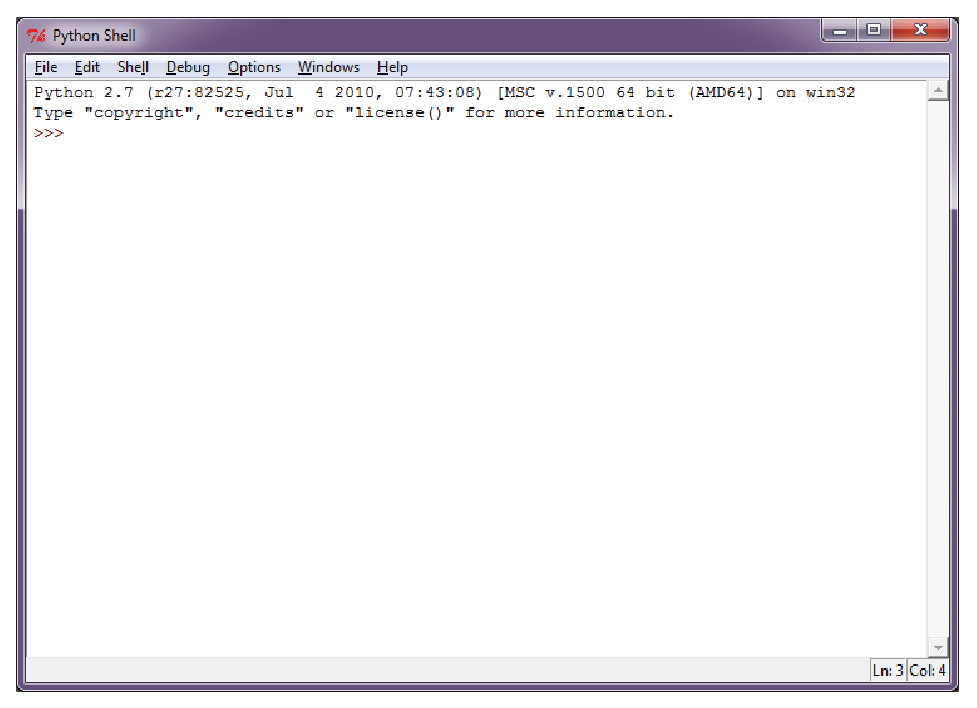
\includegraphics[scale=0.6]{fig/IDLE.eps}%
	\end{figure}
	\item Sebagai pengantar, ketikkan: 
	\begin{IDLE}
		\begin{tabbing}
		$>>>$ a = 4\\
		$>>>$ a ~~~~~~~~~~~~~~~~~~~~~~~~~~~~~~~~~~~~ \= \# \textit{Menampilkan hasil dari `a'}\\
		\textbf{4}\\
		$>>>$ a + 4\\
		\textbf{8}\\
		$>>>$ a\\
		\textbf{4}\\
		$>>>$ a = a + 4\\
		$>>>$ a\\
		\textbf{8}\\
		$>>>$ a + 1, a - 1\> \# \textit{Dua perintah dalam satu baris sekaligus}\\
		\textbf{9,7}\\
		$>>>$ a * 3, a / 2 \> \# \textit{Mengalikan dan membagi nilai `a'}\\
		\textbf{24,4}\\
		$>>>$ a \% 3, a ** 2 \> \# \textit{Modulo dan eksponen nilai `a'}\\
		\textbf{2,64}\\
		$>>>$ import math \> \# \textit{Import modul math}\\
		$>>>$ math.pi \> \# \textit{Menampilkan nilai pi (tidak semuanya)}\\
		\textbf{3.1415926535897931}\\
		$>>>$ math.sqrt(85) \> \# \textit{Akar dari nilai 85}\\
		\textbf{9.2195444572928871} \\
		$>>>$ import random \> \# \textit{Import modul random}\\
		$>>>$ random.random() \> \# \textit{Menampilkan bilangan acak 0 ~ 1}\\
		\textbf{0.3990536432569244}\\
		$>>>$ random.choice([23,54,13,44]) \> \# \textit{Memilih salah satu bilangan}\\
		\textbf{23}\\
		\end{tabbing}
	\end{IDLE}
\end{enumerate}
\end{panduan}


\begin{panduan}{Bilangan desimal}
\begin{enumerate}
	\item Buka IDLE
	\item Ketikkan:
	\begin{IDLE}
		\begin{tabbing}
			$>>>$ a = 9/2~~~~~~~~~~~~~~~~~~~~~~~~~~~~~~~~~ \= \# \textit{Melakukan pembagian}\\
			$>>>$ a \\
			4 \> \# \textit{Hasilnya merupakan bulat. Kenapa?}\\
			$>>>$  a = 9.0/2 \\
			$>>>$ a \\
			4.5 \> \# \textit{Sekarang hasilnya desimal. Kenapa?}\\
			$>>>$ a = 9/2.0 \\
			$>>>$ a \\
			4.5 \> \# \textit{Sama, hasilnya desimal. Kenapa?}\\
			$>>>$ a = float(9)/2 \> \# \textit{Melakukan casting ke float(desimal)}\\
			$>>>$ a \\
			4.5 \\
			$>>>$ b = int(a) \> \# \textit{Mengubah float(desimal) menjadi int(bulat)}\\
			$>>>$ b \\
			4\\ 
		\end{tabbing}
	\end{IDLE}
\end{enumerate}
\end{panduan}

\begin{panduan}{String}
\begin{enumerate}
	\item Buka IDLE
	\item Ketikkan:
	\begin{IDLE}
		\begin{tabbing}
		$>>>$ S = 'Spam' \\
		$>>>$ S ~~~~~~~~~~~~~~~~~~~~~~~~~~~~~~~~~~~~ \= \# \textit{Menampilkan hasil dari `S'}\\
		\textbf{'Spam'}\\
		$>>>$ len(S) \> \# \textit{Panjang dari `S'}\\
		\textbf{4}\\
		$>>>$ S[0] \> \# \textit{Karakter pertama dari `S'}\\
		\textbf{'S'}\\
		$>>>$ S[-1] \> \# \textit{Karakter terakhir dari `S'}\\
		\textbf{'m'}\\
		$>>>$ S[1:3] \> \# \textit{Irisan S dari karakter 2 sampai 4}\\
		\textbf{'pa'}\\
		$>>>$ S[1:] \> \# \textit{Irisan S dari karakter 1 sampai habis}\\
		\textbf{'pam'}\\
		$>>>$ S[:3] \> \# \textit{Irisan S dari awal sampai karakter 3}\\
		\textbf{'Spa'}\\
		$>>>$ S[:-1] \> \# \textit{Irisan S dari awal sampai karakter 1 dari belakang}\\
		\textbf{'Spa'}\\
		$>>>$ S[:] \> \# \textit{Semua isi dari S}\\
		\textbf{'Spam'}\\
		$>>>$ S + 'xyz' \> \# \textit{Penambahan karakter tetapi tidak disimpan ke `S'}\\
		\textbf{'Spamxyz}\\
		$>>>$ S * 8 \> \# \textit{Repetisi}\\
		\textbf{'SpamSpamSpamSpamSpamSpamSpamSpam'}
		\end{tabbing}
	\end{IDLE}	
\end{enumerate}
\end{panduan}

\begin{panduan}{List}
\begin{enumerate}
	\item Buka IDLE.
	\item Ketikkan:
		\begin{IDLE}
		\begin{tabbing}
		$>>>$ L = [123, 'spam', 1.23] ~~~~~~~~~~~~~~~~~~~~~ \= \\
		$>>>$ len(L) \> \# \textit{Menampilkan jumlah elemen dari `L'}\\
		\textbf{3}\\
		$>>>$ L[0]\\
		\textbf{123}\\
		$>>>$ L[:-1]\\
		\textbf{[123, 'spam']}\\
		$>>>$ L + [4,5,6]\\
		\textbf{[123, 'spam', 1.23, 4, 5, 6]}\\
		$>>>$ L.append('NI') \> \# \textit{Menambah elemen 'NI' ke `L'}\\
		$>>>$ L \\
		\textbf{[123, 'spam', 1.23, 'NI']} \\
		$>>>$ L.pop(2) \> \# \textit{Membuang elemen ketiga teratas}\\
		\textbf{1.23} \\
		$>>>$ L \\ 
		\textbf{[123, 'spam', 'NI']} \\
		$>>>$ M = [[1,2,3],[4,5,6],[7,8,9]] \> \# \textit{Matriks 3x3}
		\end{tabbing}
		\end{IDLE}	
\end{enumerate}
\end{panduan}

\begin{panduan}{Dictionaries}
\begin{enumerate}
	\item Buka IDLE.
	\item Ketikkan:
		\begin{IDLE}
		\begin{tabbing}
		$>>>$ D = {'food':'Spam', 'quantity':4, 'color':'pink'} \\
		$>>>$ D['food'] ~~~~~~~~~~~~~~~~~~~~~~~~~~~~~~~~~~~~~~~~~ \=  \# \textit{Mengambil data}
		\textbf{'Spam'} \\
		$>>>$ D['quantity'] += 1 \\
		$>>>$ D \\ 
		\textbf{\{'food': 'Spam', 'color':'pink', 'quantity':5\}} \\
		$>>>$ D = \{\} \\
		$>>>$ D \\
		\textbf{\{\}}\\
		$>>>$ D['nama'] = 'Bob' \\
		$>>>$ D['pekerjaan'] = 'programmer' \\
		$>>>$ D['umur'] = 40 \\
		$>>>$ D \\
		\textbf{\{'umur': 40, 'pekerjaan':'programmer', 'nama':'Bob'\}}
		\end{tabbing}
		\end{IDLE}	
\end{enumerate}
\end{panduan}

\subsection{IDE}
Untuk input dari keyboard, python menggunakan sintaks seperti di Listing \ref{lst:inputPython}
\begin{listprog}{Input di Python (input.py)}
	\label{lst:inputPython}
	\begin{lstlisting}[language=Python]
	umur = input("Berapa umur anda?")
	print "Umur anda adalah: ", umur, "tahun."
	\end{lstlisting}
\end{listprog}
\begin{panduan}{Input}
\begin{enumerate}
	\item Buka \textbf{IDLE atau PyScripter for Python 3.3}
	\item Ketikkan Listing \ref{lst:inputPython}.
	\item Tekan CTRL-F9 untuk jalankan.
	\item Save sebagai input.py
\end{enumerate}
\end{panduan}
%\chapter{Lampiran: QQQ}\label{ch:app2}
\section{Variabel}
Variabel merupakan tempat penyimpanan data. 


\end{document}
